\title{CS 383 - Machine Learning}
\author{
Assignment 2 - Clustering\\
Summer 2017\\
Amir Omidi
}
\date{}
\documentclass[12pt]{article}
    \usepackage[margin=0.7in]{geometry}
    \usepackage{graphicx}
    \usepackage{float}
    \usepackage{amsmath}
    
    
\begin{document}
\maketitle

\newpage
\section{Programming Questions}
\subsection{Basic k-Means Clustering}
\subsubsection{Initial Setup Visualization}
The following figure displays the initial data visualization.

\begin{figure}[h!]
    \begin{center}
        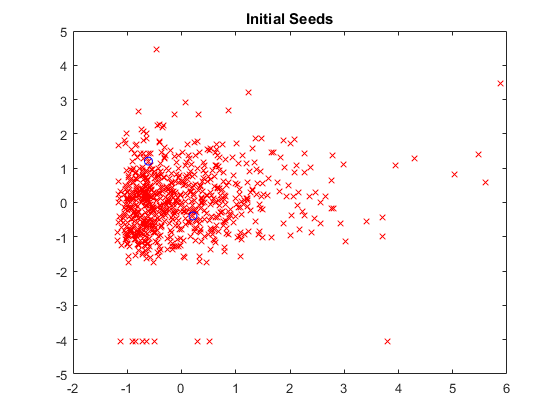
\includegraphics[scale=1.2]{TQ2_a.png}
        \caption{Initial setup visualization}
    \end{center}
\end{figure}
Code: (Yes; the function is called kmeme on purpose :D)
\begin{verbatim}
    otherData = kmeme(newData(:,8:-1:7), 2, 1, 2);
\end{verbatim}
\newpage

\subsubsection{Initial Cluster Assignment}
The following figure displays the initial clustering of the data.

\begin{figure}[h!]
    \begin{center}
        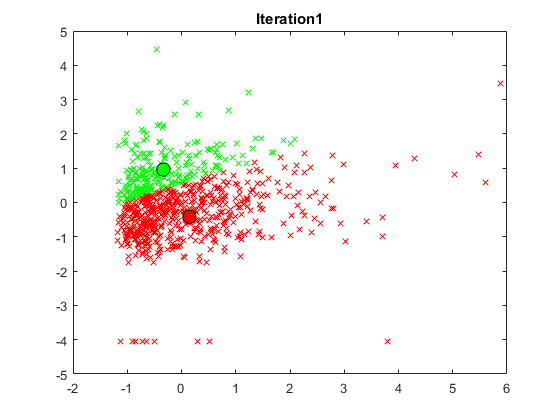
\includegraphics[scale=1.2]{TQ2_b.png}
        \caption{Initial clustering of data}
    \end{center}    
\end{figure}

\newpage

\subsubsection{Final Cluster Assignment}
The following figure displays the final clustering of the data.

\begin{figure}[h!]
    \begin{center}
        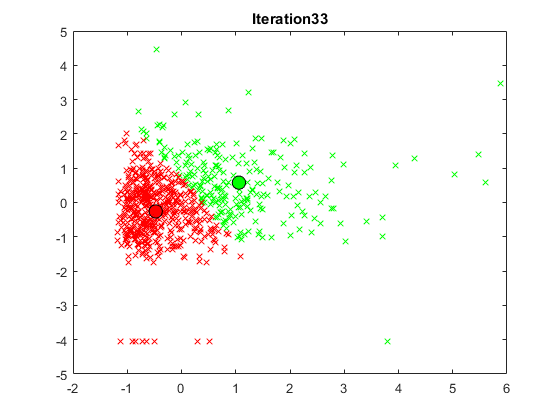
\includegraphics[scale=1.2]{TQ2_c.png}
        \caption{Final clustering of data}
    \end{center}    
\end{figure}


\newpage

\subsection{Flexible k-Means Clustering}
\subsubsection{Sample 1}
This sample of data is the clustering of all the data with $k=2$, but displaying the 6th and 7th features only (The BMI and Pedigree values).
\\[0.1 in]
\textbf{Initial Seeds}
\\[0.1 in]
The inital seeds are ofcourse going to be the same as section 1.1.1:
\begin{figure}[h!]
    \begin{center}
        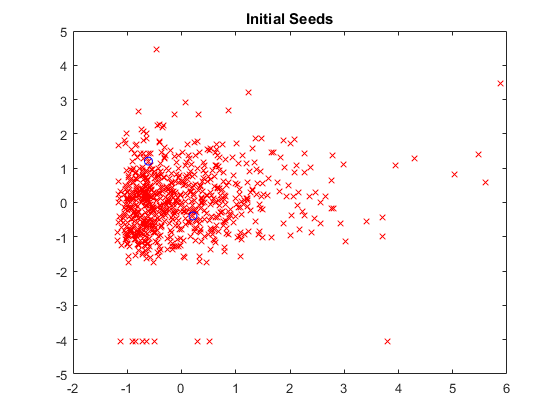
\includegraphics[scale=1.2]{TQ2_a.png}
        \caption{Initial setup visualization}
    \end{center}
\end{figure}

\newpage
\noindent
\textbf{Initial clustering assignments}
\\[0.1 in]
The inital clustering for this data.
\begin{figure}[h!]
    \begin{center}
        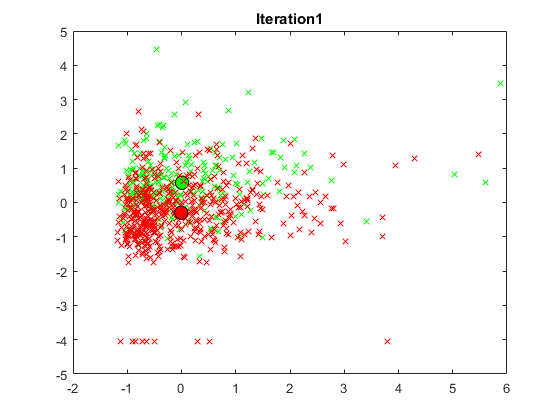
\includegraphics[scale=1.2]{TQ3_1_b.png}
        \caption{Initial clustering of data}
    \end{center}    
\end{figure}
\\
As you can see it looks quite different from 1.1.2.

\newpage
\noindent
\textbf{Final clustering assignments}
\\[0.1 in]
The final clustering for this data.
\begin{figure}[h!]
    \begin{center}
        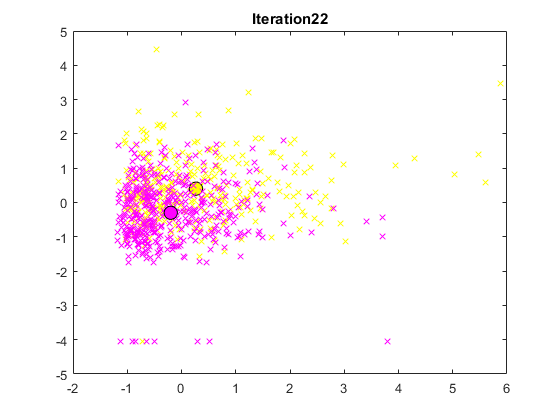
\includegraphics[scale=1.2]{TQ3_1_c.png}
        \caption{Final clustering of data}
    \end{center}    
\end{figure}


\newpage

\subsubsection{Sample 2}
This sample of data is the clustering of all the data with $k=4$, but displaying the 2nd and 3rd features only.

\noindent
The code to run this:

\begin{verbatim}
    otherData = kmeme(newData, 4, 4, 3)
\end{verbatim}

The final clustering for this data.
\begin{figure}[h!]
    \begin{center}
        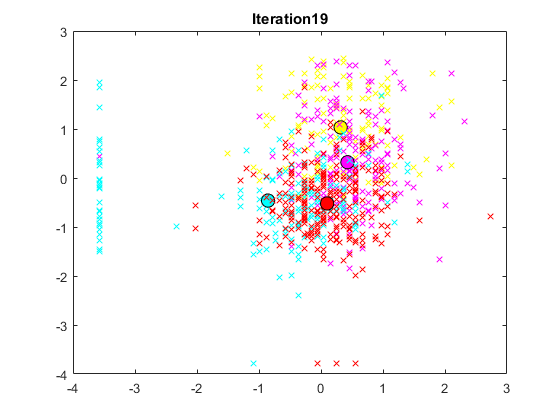
\includegraphics[scale=1.2]{TQ3_2.png}
        \caption{Final clustering of data}
    \end{center}    
\end{figure}

\newpage

\subsubsection{Sample 3}
This sample of data is the clustering of all the data with $k=5$, but displaying the 1st and 2nd features only.

\noindent
The code to run this:

\begin{verbatim}
    otherData = kmeme(newData, 5, 2, 3);
\end{verbatim}

The final clustering for this data.
\begin{figure}[h!]
    \begin{center}
        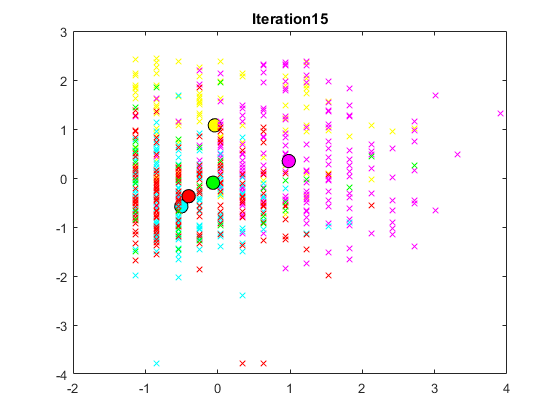
\includegraphics[scale=1.2]{TQ3_3.png}
        \caption{Final clustering of data}
    \end{center}    
\end{figure}

\newpage

\subsubsection{Sample 4}
This sample of data is the clustering of all the data with $k=7$, but displaying the 5th and 7th features only.

\noindent
The code to run this:

\begin{verbatim}
    otherData = kmeme(newData, 7, 8, 6);
\end{verbatim}

The final clustering for this data.
\begin{figure}[h!]
    \begin{center}
        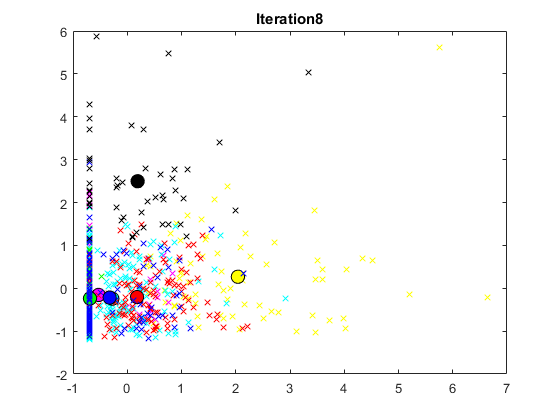
\includegraphics[scale=1.2]{TQ3_4.png}
        \caption{Final clustering of data}
    \end{center}    
\end{figure}

\end{document}

